\documentclass{article}

\usepackage{Vor2018skil}

\title{Tölvunarfræði 2, \semester \\ Skilaverkefni 3}
\author{}

\begin{document}
\maketitle
\hypersetup{pdftitle={Tölvunarfræði 2 - Skilaverkefni 3}}

Skila skal þessum verkefnum á \href{https://gradescope.com/courses/14122}{Gradescope}.

Þegar forriti er skilað inn til yfirferðar er mikilvægt að láta \textbf{niðurstöðurnar fylgja}. Öllum forritskóða skal skila framsettum með jafnbilaletri. Hann þarf að vera afritanlegur úr .pdf skjalinu. Vönduð framsetning og læsilegur kóði er hluti af verkefninu.

Athugið að fyrstu tvö verkefni þessarar viku eru verkefni í \textbf{Java}. Gert er ráð fyrir að forritun í Java sé að mestu leyti þekkt úr Tölvunarfræði 1. Mikilvægt er að setja upp Java-þýðanda sem allra fyrst. Verkefni næstu viku krefjast þess líka að forritssafn kennslubókarinnar (algs4.jar) sé sett upp. Sjá \href{http://algs4.cs.princeton.edu/code/}{leiðbeiningar á síðu bókarinnar}.
\question

Aftur er gefinn vísir að \href{https://raw.githubusercontent.com/Ernir/kennsluefni/master/T2/Code/w4/Fraction.java}{klasa sem táknar almenn brot}. Þar á eftir að útfæra tvær gerðir samanburða - með \texttt{equals} aðferð, sem reiknar hvort að brotin tákni sömu stærð og með \texttt{compareTo}, sem skilgreinir röðun.

Klárið útfærsluna. Ekki breyta \texttt{main} fallinu sem er gefið eða hausum fallanna sem á að útfæra. Útskriftin ætti að vera:

\begin{verbatim}
$ java Fraction
p.equals(p): true
p.equals(r): true
r.equals(p): true
p.equals(r): true
r.equals(t): true
p.equals(t): true
t.equals(null): false
q.compareTo(q): 0
r.compareTo(q): 1
q.compareTo(r): -1
r.compareTo(q): 1
q.compareTo(s): 1
r.compareTo(s): 1
\end{verbatim}

\paragraph{Ábending:} Hægt er að lesa um kröfur sem gerðar eru til \texttt{equals} á \href{https://docs.oracle.com/javase/7/docs/api/java/lang/Object.html#equals(java.lang.Object)}{síðu Oracle} og á bls. 102 í kennslubók. Hægt er að lesa um \texttt{compareTo} á \href{https://docs.oracle.com/javase/8/docs/api/java/lang/Comparable.html}{síðu Oracle} og á bls. 246-247 í kennslubók.

\question

Gefinn er byrjun á fjölnota Java-klasanum \href{https://raw.githubusercontent.com/Ernir/kennsluefni/master/T2/Code/w4/SinglyLinkedList.java}{\texttt{SinglyLinkedList}} sem skal uppfylla eftirfarandi skil:

\begin{center}
\begin{tabularx}{\linewidth}{rlX}
\toprule
Skilar&Notkun&Lýsing\\
\midrule
-&\texttt{SinglyLinkedList()}& Smiður, upphafsstillir tóman lista\\
\texttt{boolean}&\texttt{isEmpty()}&Skilar sönnu sé listinn tómur, annars ósönnu\\
\texttt{int}&\texttt{size()}&Skilar fjölda staka í listanum\\
\texttt{String}&\texttt{toString()}&Skilar snyrtilegri framsetningu á gögnum listans\\
\texttt{T}&\texttt{get(int index)}&Skilar gildi staks númer \texttt{index} í listanum\\
\texttt{void}&\texttt{insert(int index, T data)}&Setur stak með gögnin \texttt{data} á stað \texttt{index} í listanum, gögn sem á eftir koma hliðrast í átt að enda listans\\
\bottomrule
\end{tabularx}
\end{center}
Klárið útfærsluna. Ekki breyta \texttt{main} fallinu sem er gefið eða hausum fallanna sem á að útfæra. Útskriftin ætti að vera:

\begin{verbatim}
$ java SinglyLinkedList
[ 2 ]
[ 1 2 ]
[ 1 2 4 ]
[ 1 2 3 4 ]
list1.get(0): 1
list1.get(1): 2
list1.get(2): 3
list1.get(3): 4
Kall á list1.get(-1) mistókst réttilega
Kall á list1.get(list1.size()) mistókst réttilega
[ A B C D ]
\end{verbatim}

\question
Hringvísanir valda oft vandræðum við forritun. T.d. er auðvelt að skilgreina forrit óvart hvert út frá öðru (eins og $f(x) = g(x), g(x) = h(x), h(x) = f(x)$). Til eru reiknirit sem sérstaklega eru hönnuð til að þefa uppi hringvísanir.

Reiknirit sem kennt er við ``hérann og skjaldbökuna'' er hægt að nota til að uppgötva hringvísanir í eintengdum listum (sjá mynd \ref{fig:circular-list}).

\begin{figure}
    \caption{Listi sem hefur verið eyðilagður með hringvísun}
    \label{fig:circular-list}
    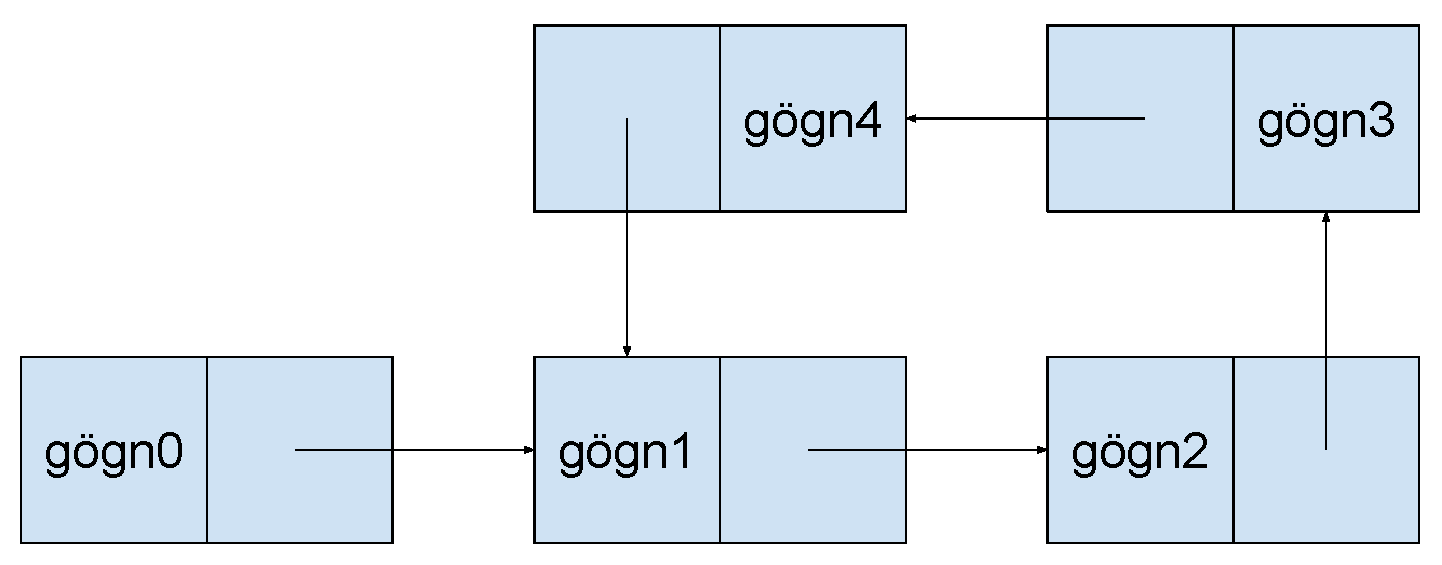
\includegraphics[width=\textwidth]{circular-list}
\end{figure}

Reikniritið notar tvo benda, annar er hérinn og hinn er skjaldbakan. Báðir byrja í haus listans en færast á mismunandi hraða. Í hverri ítrun reikniritsins færist hérinn fram um tvo hnúta en skjaldbakan fram um einn. Listinn inniheldur hringvísun þá og því aðeins að bendarnir vísi einhvern tímann á sama hnút eftir að ítrun hefst. 

Gefin er \href{https://raw.githubusercontent.com/Ernir/kennsluefni/master/T2/Code/w4/cycledetection.cpp}{beinagrind}. Klárið að útfæra \texttt{hasCycle} aðferðina með reikniriti hérans og skjaldbökunnar. Ekki breyta \texttt{main} fallinu sem er gefið. Útskriftin ætti að vera á forminu:

\begin{verbatim}
$ ./cycledetection
Listinn er af lengd 781
Listinn inniheldur hring
\end{verbatim}

\vfill
%
\includegraphics[width=0.5\linewidth]{hi-von-logo}
\end{document}